\chapter{Apartado B}
\label{chapter:tarea_b}

En este apartado se trabajará en la corrección de la distorsión debido a lentes de ojo de pez. Primero se calibrará una cámara con este tipo de lente. Posteriormente se utilizarán estos parámetros de calibración para corregir la distorsión de una de las imágenes de calibración. La Figura \ref{fig:fisheye_camera} muestra un ejemplo (no digital) de este tipo de dispositivos \footnote{ \href{https://commons.wikimedia.org/wiki/File:Fisheye-Nikkor\_Auto\_6mm\_f2.8\_lens\_2015\_Nikon\_Museum.jpg}{Morio, CC BY-SA 4.0 <https://creativecommons.org/licenses/by-sa/4.0>, via Wikimedia Commons} https://commons.wikimedia.org/wiki/File:Fisheye-Nikkor\_Auto\_6mm\_f2.8\_lens\_2015\_Nikon\_Museum.jpg}.

\begin{figure}[h]
    \centering
    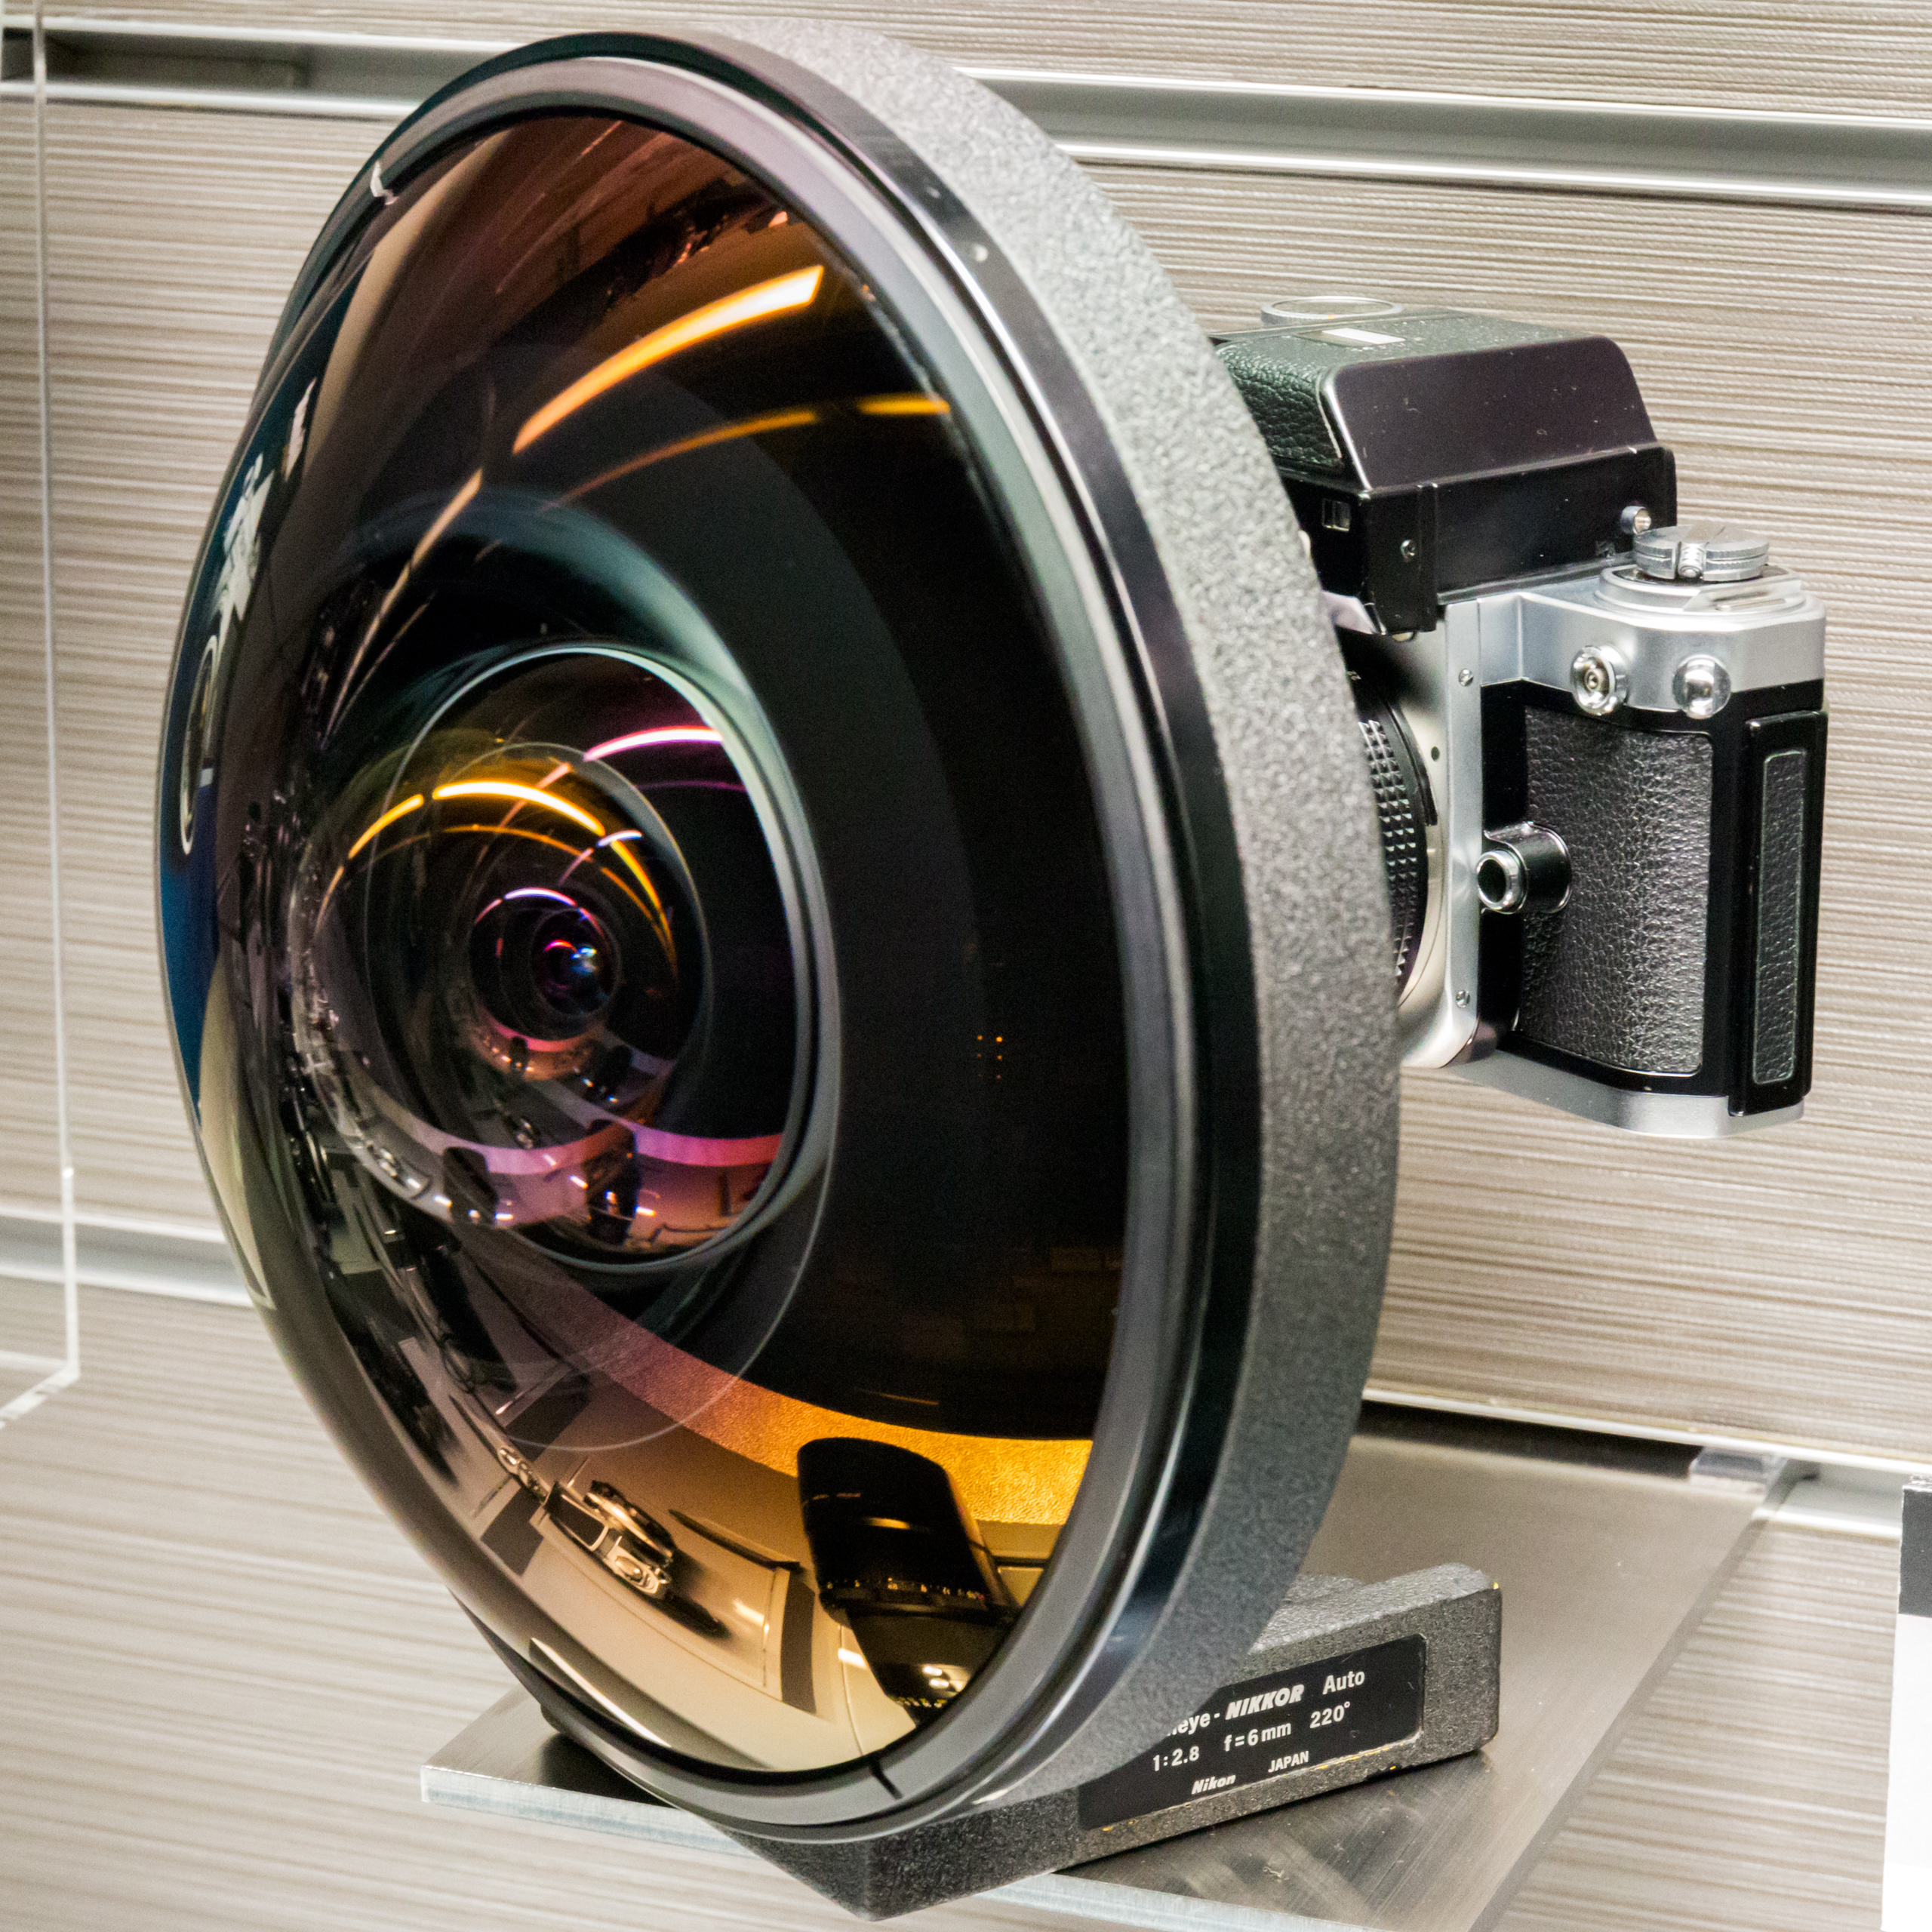
\includegraphics[width=0.45\textwidth]{Lab_1/template/figures/ojo_pez.jpg}
    \caption{Lente ojo de pez.}
    \label{fig:fisheye_camera}
\end{figure}

Para este ejercicio, las imágenes de calibración se encuentran en la carpeta \textit{fisheye}. De nuevo, se recomienda consultar la documentación de la función utilizada para calibrar y sus argumentos: \texttt{cv2.fisheye.calibrate()} \footnote{Doc. \href{https://docs.opencv.org/4.x/db/d58/group\_\_calib3d\_\_fisheye.html\#gad626a78de2b1dae7489e152a5a5a89e}{cv2.fisheye.calibrate()} https://docs.opencv.org/4.x/db/d58/group\_\_calib3d\_\_fisheye.html\#gad626a78de2b1dae7489e152a5a5a89e1}. 

Una vez hecho ese ejercicio mental, deberá seguir los pasos de este enunciado para conseguir un modelo de cámara y corregir la distorsión:

\section*{Tarea B.1: Carga de Imágenes}
\addcontentsline{toc}{section}{Tarea B.1: Carga de Imágenes}
Reutilice el método \texttt{load\_images()} para cargar las imágenes de la carpeta \texttt{fisheye}. En esta ocasión, puede apoyarse en el método \texttt{glob.glob('path\_to\_folder/*.jpg')} para obtener una lista con la ruta de todas las imágenes de interés.


\section*{Tarea B.2: Detección de esquinas de las imágenes}
\addcontentsline{toc}{section}{Tarea B.2: Detección de esquinas de las imágenes}
Utilice los métodos \texttt{cv2.findChessboardCorners()} y \texttt{cv2.cornerSubPix()} para obtener las esquinas del tablero de todas las imágenes. Recuerde que para utilizar \texttt{cv2.cornerSubPix()} deberá pasar las imágenes a escala de grises y definir \texttt{subpix\_criteria}.

Asegúrese de que el output de esta tarea contenga solo los casos en los que las detecciones son adecuadas.

\section*{Tarea B.3: Obtención de coordenadas del tablero}
\addcontentsline{toc}{section}{Tarea B.3: Obtención de coordenadas del tablero}
Reutilice el método \texttt{get\_chessboard\_points()} para obtener las coordenadas del nuevo tablero. Para obtener el número de filas y columnas, abra de forma manual una de las imágenes. La longitud de cada cuadrado en los patrones es de 30 mm.

De nuevo, tenga en cuenta que deberá proporcionar una lista que contenga los puntos para todas las imágenes con detecciones correctas.

\textbf{Nota}: La función de calibración espera que cada vector asociado a cada imagen tenga el siguiente formato: $(n, 1, 3)$, siendo $n$ el número de puntos detectados.

\section*{Tarea B.4: Definición de parámetros para calibración}
\addcontentsline{toc}{section}{Tarea B.4: Definición de parámetros para calibración}

Defina los parámetros necesarios para llamar a la función \texttt{cv2.fisheye.calibrate()}:

\begin{itemize}
    \item \texttt{calibration\_flags}: Configura el método de calibración.
    \item \texttt{intrinsics}: Matriz de intrínsecos.
    \item \texttt{distortion}: Vector con coeficientes de distorsión.
    \item \texttt{rotations}: Vectores de rotación.
    \item \texttt{traslations}: Vectores de traslación.
\end{itemize}


\section*{Tarea B.5: Calibración}
\addcontentsline{toc}{section}{Tarea B.5: Calibración}

Utilice el método \texttt{cv2.fisheye.calibrate()} y visualice el valor de \texttt{intrinsics}, \texttt{distortion}.

\newpage
\section*{Preguntas}
\addcontentsline{toc}{section}{Preguntas}

\vspace{5mm}
\begin{tcolorbox}[colback=gray!10, colframe=gray!30, coltitle=black, title=Pregunta B.1, halign=left]
Una vez calibrada la cámara con lente de ojo de pez, tiene acceso a la matriz de intrínsecos y los coeficientes de distorsión. Con estos valores y con ayuda de las funciones \texttt{cv2.fisheye.initUndistortRectifyMap()} y \texttt{cv2.remap()} podrá eliminar la distorsión de las imágenes tomadas por este tipo de cámaras. En el notebook encontrará ayuda para trabajar con la función \texttt{cv2.fisheye.initUndistortRectifyMap()}. Sin embargo, en el caso de \texttt{cv2.remap()} \footnotemark deberá utilizar la documentación para obtener la imagen solicitada. Para obtener toda la puntuación de este apartado, facilite el valor de la matriz de intrínsecos y los coeficientes de distorsión de la cámara. Además, adjunte las imágenes sin distorsión de las 2 primeras imágenes de la carpeta \textit{fisheye}.
\end{tcolorbox}

\footnotetext{Doc. \href{https://docs.opencv.org/4.x/da/d54/group\_\_imgproc\_\_transform.html\#gab75ef31ce5cdfb5c44b6da5f3b908ea4}{cv2.remap()} https://docs.opencv.org/4.x/da/d54/group\_\_imgproc\_\_transform.html\#gab75ef31ce5cdfb5c44b6da5f3b908ea4}


